\chapter{Oversampling para clasificación de series temporales}
En este capítulo se describirán diferentes algoritmos de oversampling que se utilizarán más adelante en el estudio. Con dichos algoritmos de oversampling se busca mejorar el rendimiento de los modelos que se probarán en el estudio. Los algoritmos que a continuación se van a describir son SMOTE, MWMOTE y ADASYN.

\section{SMOTE}
SMOTE (Synthetic Minority Oversampling Technique) es uno de los algoritmos de oversampling más utilizados a día de hoy. Este algortimo fue inventado en 2002 y actualmente se considera como uno de los algoritmos en el estado del arte del oversampling.\newline

Para balancear los datos de las diferentes clases, SMOTE propone generar instancias de la clase minoritaria de forma sintética. Para ello, SMOTE utiliza las instancias de la clase minoritaria para generar nuevas instancias de dicha clase con características parecidas a las ya existentes.\newline

Para conseguir dicho objetivo SMOTE sigue el siguiente proceso, elige una instancia de la clase minoritaria cualquiera, tras esto se buscan sus $K$ vecinos más cercanos que sean también de la clase minoritaria; dicho parámetro $K$ se puede cambiar y afecta a como son las instancias generadas sintéticamente; si por ejemplo su valor fuera $K=1$, las instancias se generan a partir de dos instancias de la clase minoritaria, esto hace que las características de dichas instancias nuevas sean muy parecidas a las de las instancias que se han utilizado; en cambio si $K$ tiene un valor muy grande entonces las instancias generadas tienen menos parecido a las instancias con las que se han generado.\newline

Una vez se han obtenido el número de vecinos elegido, la nueva instancia se genera como una combinación de las instancias que se utilizan, por ejemplo si $K=1$, la nueva instancia se generaría como la media de los valores de dichas instancias.\newline

\begin{figure}[h]
	\centering
	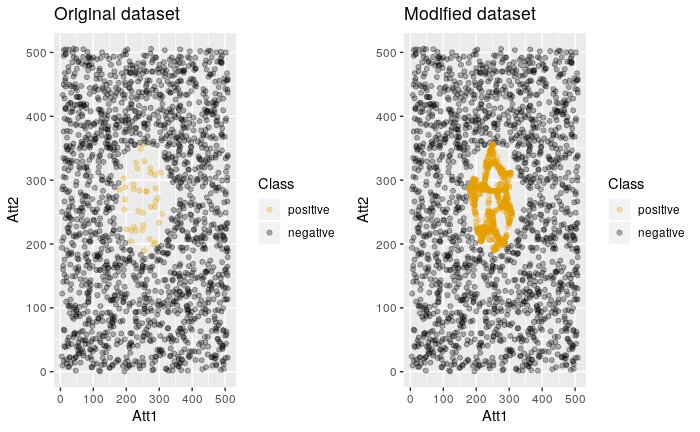
\includegraphics[width=100mm]{imagenes/SMOTE_comparison.png}
	\label{fig:12}
	\caption{Ejemplo de generación de instancias con SMOTE.}
\end{figure}
\verticalspace

Uno de los principales problemas de SMOTE es que no es bueno utilizarlo cuando las clases del conjunto de datos están mezcladas, es decir, dentro de los datos de la clase mayoritaria puede haber un pequeño conjunto de la clase minoritaria (la cual podría considerarse ruido); si utilizaramos SMOTE, el número de instancias de ese conjunto sería mayor y esto afectaría al rendimiento de un modelo. Por ello, antes de utilizar este método es bueno realizar otro tipo de preprocesamientos como limpieza de ruido, imputación de valores perdidos, etc...
\newpage
\section{MWMOTE}
MWMOTE (Mayority Weighted Minority Oversampling Technique) se trata de una modificación del algoritmo SMOTE para evitar de instancias ruidosas.\newline

El objetivo de este algoritmo es mejorar la forma de seleccionar instancias y la forma de generar las instancias sintéticas. Para ello este algoritmo cuenta con tres fases.\newline

En la primera fase se identifican los ejemplos de la clase minoritaria, a este conjunto lo podemos llamar $S_{min}$; que son más difíciles de aprender, para ello se genera un conjunto con dichos ejemplos al que llamaremos $S_{imin}$. Para generar este conjunto el algoritmo elimina todas aquellas instancias de $S_{min}$ que no tenga ninguna instancia de $S_{min}$ en su vecindario; para calcular el vecindario se utiliza el mismo proceso que para SMOTE. Una vez eliminados, se calculan aquellas instancias que son fronterizas con un conjunto de datos de la clase mayoritaria, estas instancias son las que forman $S_{imin}$.\newline

En la segunda fase, cada uno de los ejemplos de $S_{imin}$ se le agrega un peso dependiendo de la importancia de dicho ejemplo dentro de el conjunto de datos de $S_{min}$. Para ello se calcula la cantidad de información que se obtiene de cada uno de los puntos, esta medida se calcula teniendo en cuenta como de cercano está cada instancia al conjunto de datos de la clase mayoritaria. Por último, una vez calculado el peso de cada instancia se le asocia una probabilidad a dicho peso.\newline

En la tercera fase, el algoritmo genera instancias sintéticas a partir de $S_{imin}$ usando dicho peso y los añade al conjunto de datos de la clase minoritaria. Para generar dichas instancias, se detectan diferentes clústers dentro de $S_{min}$ y se por cada instancia que se genera se elige un elemento del conjunto $S_{imin}$ $x$, se elige otra instancia $y$ de $S_{min}$ que se encuentre en el mismo clúster que $x$ y se genera una nueva instancia de la siguiente forma: $ s = x + \alpha \times (y-x)$. \newline

\begin{figure}[h]
	\centering
	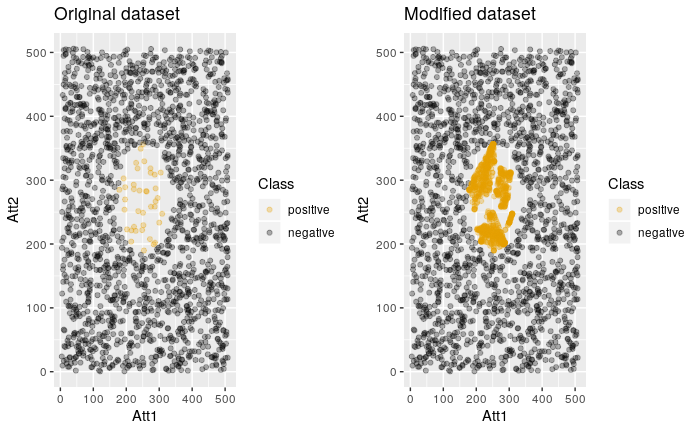
\includegraphics[width=100mm]{imagenes/MWMOTE_comparison.png}
	\label{fig:13}
	\caption{Ejemplo de generación de instancias con MWMOTE.}
\end{figure}
\verticalspace
\newpage
\section{ADASYN}
ADASYN (Adaptive Synthetic Sampling) se trata de un algoritmo motivado por SMOTE. Al igual que el algoritmo de la sección anterior, propone otra forma de generar instancias. El objetivo principal de este algoritmo es reducir el sesgo entre ambas clases mientras aprende de forma adaptada. el procedimiento que sigue este algoritmo es el siguiente.\newline

Primero, calcula el ratio entre instancias de la clase minoritaria y mayoritaria; este ratio después se utiliza para calcular el número de instancias de la clase minoritaria a generar.\newline

Tras esto, por cada instancia perteneciente a la clase minoritaria, se calcula su valor $r_i$, este valor indica la dominancia de ejemplos de la clase mayoritaria en el vecindario de esta instancia; a valores mayores de esta medida es más difícil aprender sobre dicha instancia. Una vez calculadas todas las medidas se normalizan.\newline

Una vez calculadas todas las medidas $r_i$, se calcula el número de instancias a generar en el vecindario de dicha instancia de la siguiente manera: $G_i = G r_i$; donde $G$ es el número de instancias a generar que se calculó al principio.\newline
\newpage

Por último, cada una de las instancias en un vecindario $i$ se genera de la siguiente forma: se selecciona una instancia del vecindario, $x_i$; después se selecciona de forma aleatoria otra instancia vecina a la instancia $x_i$, la llamaremos $x_{zi}$; por último se calcula un número aleatorio entre 0 y 1 y se calcula la nueva instancia como la siguiente fórmula: $ s_i = x_i + (x_{zi}-x_i)\lambda$.\newline

\begin{figure}[h]
	\centering
	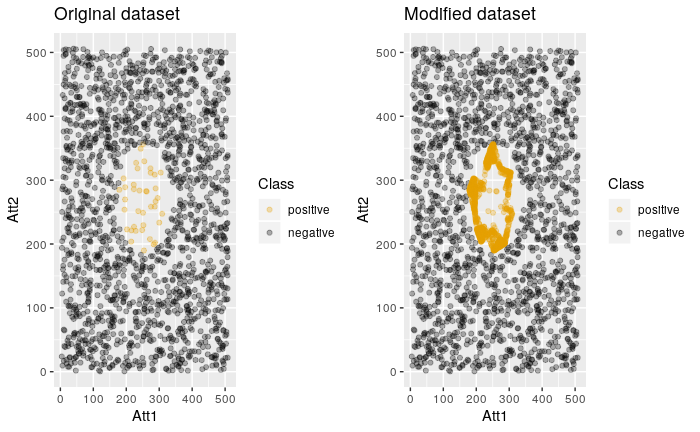
\includegraphics[width=100mm]{imagenes/ADASYN_comparison.png}
	\label{fig:14}
	\caption{Ejemplo de generación de instancias con ADASYN.}
\end{figure}
\verticalspace

Uno de los problemas de ADASYN es que puede generar instancias en vecindarios donde el número de instancias de la clase minoritaria es muy reducida, produciendo ruido.
